\newpage
\section{Pensando como economista}
\subsection{Modelos económicos}
Los economista utilizan modelos creados bajo ciertos supuestos para simplificar la realidad con el fin de mejorar nuestra comprensión del mundo. Dos de los modelos económicos más básicos son:
\begin{itemize}
	\item El diagrama de flujo circular: explicar en términos generales cómo se organiza la economía y la manera en que los diferentes acotres interactúan. Es un modelo visual de la economía que muestra cómo el dinero fluyen a través de los mercados entre los hogares y las empresas.
	\begin{figure}[h]
		\centering
		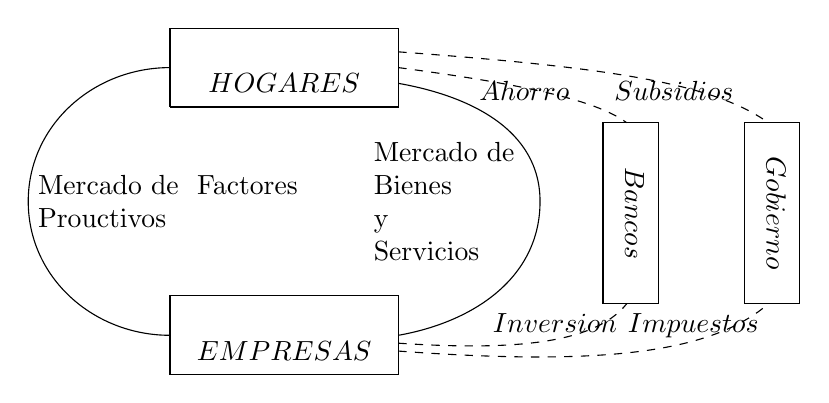
\begin{tikzpicture}		
\node [black] at (3.25, 0.3) {$EMPRESAS$};		
\node [black] at (3.25, 3.7) {$HOGARES$};	
\node [black] at (6.3, 3.6) {$Ahorro$};
\node [black] at (8.2, 3.6) {$Subsidios$};
\node at (7.7,2.05){\rotatebox{-90}{$Bancos$}};	
\node at (9.5, 2.05){\rotatebox{-90}{$Gobierno$}};
\node at (0, 2.2) [align = left, right] {Mercado de \ Factores \\ Prouctivos};
\node at (6.3, 2.2) [align = left, left] {Mercado de \\ Bienes \\ y \\ Servicios};
\draw [black] (1.8, 0) -- (4.7, 0) -- (4.7, 1) -- (1.8, 1) -- (1.8, 0);
\draw [black] (1.8, 3.4) -- (4.7, 3.4) -- (4.7, 4.4) -- (1.8, 4.4) -- (1.8, 3.4);	
\draw [black] (7.3, 0.9) -- (8, 0.9) -- (8, 3.2) -- (7.3, 3.2) -- (7.3, 0.9);		
\draw [black] (9.1, 0.9) -- (9.8, 0.9) -- (9.8, 3.2) -- (9.1, 3.2) -- (9.1, 0.9);		
\draw [black] (1.8, 3.9) to [out=-180, in=90] (0, 2.2) to [out=-90, in=180] (1.8, 0.5);
\draw [black] (4.7, 0.5) to [out=10, in=-90] (6.5, 2.2) to [out=90, in=-10] (4.7, 3.7);
\draw [black] [dashed] (4.7, 0.4) ..controls (6.2, 0.3) and (7.2, 0.4) ..(7.6, 0.9) node [below left] {$Inversion$};
\draw [black] [dashed] (4.7, 0.3) ..controls (7.4, 0.1) and (8.7, 0.3) ..(9.4, 0.9) node [below left] {$Impuestos$};
\draw [black] [dashed] (4.7, 3.9) ..controls (6.2, 3.7) and (7.2, 3.5) ..(7.6, 3.2);
\draw [black] [dashed] (4.7, 4.1) ..controls (7.4, 3.9) and (8.7, 3.7) ..(9.4, 3.2);
		\end{tikzpicture}
		\caption{Diagrama de Flujo Circular moderno}
	\end{figure}
	\item La frontera de posibilidades de producción: la herramienta matemática más simple en economía es un gráfico que muestra las combinaciones de producción que la economía puede generar dados los factores de producción y la tecnología disponible. Por tanto un cambio en los factores productivos o tecnologicos genera otra frontera de producción.
	\\
	La frontera de posibilidades de producción se abrevia FPP. Entiendase esta como la disyuntiva entre producir un bien u el otro. Dicho eso, el coste de producción de fabricar el bien X, se expresara en bienes no producidos Y.
	\endgroup
	\begin{figure}[h]
		\centering
		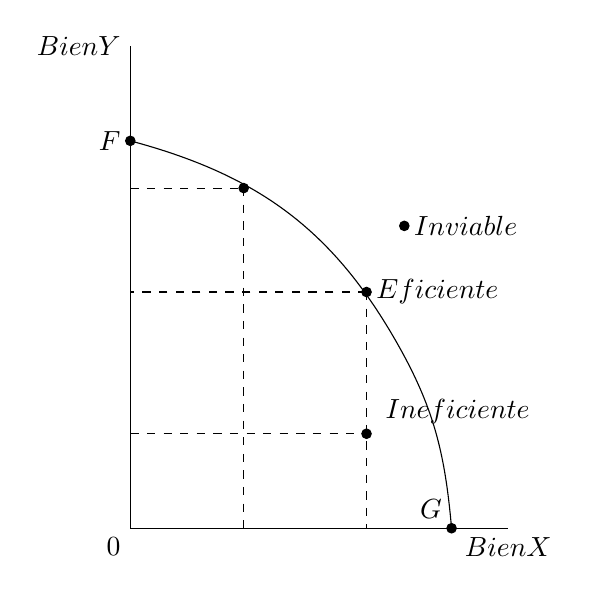
\begin{tikzpicture}[scale=1.2]
		\draw (0,5.1) node [left] {$Bien Y$} -- (0,0) node [below left] {$0$} -- (4,0) node [below] {$Bien X$};
		\draw (0,4.1) to [out=-15, in=120] (2.8,2) to [out=-60, in=95] (3.4,0);
		\draw [dashed] (1.2,3.6) -- (1.2,0);
		\draw [dashed] (0,3.6) -- (1.2,3.6);
		\draw [dashed] (2.5,2.5) -- (2.5,0);
		\draw [dashed] (2.5,2.5) -- (0,2.5);
		\draw [dashed] (0,1) -- (2.6,1);
		\node [above right] at (2.6,1) {$Ineficiente$};
		\draw [fill] (2.5,1) circle [radius=.05];	
		\node [left] at (0,4.1) {$F$};
		\draw [fill] (0,4.1) circle [radius=.05];
		\node [above left] at (3.4,0) {$G$};
		\draw [fill] (3.4,0) circle [radius=.05];
		\node [right] at (2.5,2.5) {$Eficiente$};	
		\draw [fill] (2.5,2.5) circle [radius=.05];	
		\node [right] at (2.9,3.2) {$Inviable$};
		\draw [fill] (2.9,3.2) circle [radius=.05];		
		\draw [fill] (1.2,3.6) circle [radius=.05];
		
		\end{tikzpicture}
		
		\caption{Frontera de Posibilidades de Produccion}
		
	\end{figure}

\begin{center}
	\begin{tabular}{l|l}
		{\bf Microeconomía}&Se centra en las partes individuales de la economía.\\ \hline
		{\bf Macroeconomía}&Mira a la economía en su conjunto
	\end{tabular}
\end{center}

\subsection{Los economistas como asesores políticos}
Cuando los economistas tratan de explicar como es el mundo se les puede tratar como \underline{científicos}. Sin embargo, cuando un economista intenta darle forma al mundo, son \underline{asesores políticos}. Debido a lo anterior ambos usan el lenguaje de manera distinta. Para eso existen diferentes tipos de afirmaciones:

\begingroup
\setlength{\tabcolsep}{5pt} % Default value: 6pt
\renewcommand{\arraystretch}{1.5} % Default value: 1
\begin{center}
\begin{tabular}{p{1.7cm}|p{11cm}}
{\bf Positiva}& Es descriptiva y se refiere a cómo es el mundo. Esta se tiende a usar más cuando el area es mas cientifica\\ \hline
{\bf Normativa}& Es prescriptiva y se refiere a cómo deberia de ser el mundo. Esta se tiende a usar más cuando buscamo políticas que son deseables
\end{tabular}
\end{center}
\endgroup

Debido a que todos utilizamos el lenguaje de manera distinta, los economistas tienden a discrepar entre sí. Estas discrepancias se pueden causar por no estar de acuerdo con la validez de otras teorías positivas, pero tambien se pueden causar porque cada economista puede tener sus propios valores. Y con ello teber distintas viciones normativas de lo que la política económica devería tratar de lograr.
